% --------------------------------------------------------------
% This is all preamble stuff that you don't have to worry about.
% Head down to where it says "Start here"
% --------------------------------------------------------------
 
\documentclass[12pt]{article}
\usepackage{enumitem}
\usepackage{xcolor}
\usepackage[margin=1in]{geometry} 
\usepackage{amsmath,amsthm,amssymb}
\usepackage[colorlinks,allcolors=blue]{hyperref}
\usepackage{cleveref}
\newcommand{\N}{\mathbb{N}}
\newcommand{\Z}{\mathbb{Z}}
\usepackage{graphicx}
\newenvironment{theorem}[2][Theorem]{\begin{trivlist}
\item[\hskip \labelsep {\bfseries #1}\hskip \labelsep {\bfseries #2.}]}{\end{trivlist}}
\newenvironment{lemma}[2][Lemma]{\begin{trivlist}
\item[\hskip \labelsep {\bfseries #1}\hskip \labelsep {\bfseries #2.}]}{\end{trivlist}}
\newenvironment{exercise}[2][Exercise]{\begin{trivlist}
\item[\hskip \labelsep {\bfseries #1}\hskip \labelsep {\bfseries #2.}]}{\end{trivlist}}
\newenvironment{problem}[2][Problem]{\begin{trivlist}
\item[\hskip \labelsep {\bfseries #1}\hskip \labelsep {\bfseries #2.}]}{\end{trivlist}}
\newenvironment{question}[2][Question]{\begin{trivlist}
\item[\hskip \labelsep {\bfseries #1}\hskip \labelsep {\bfseries #2.}]}{\end{trivlist}}
\newenvironment{corollary}[2][Corollary]{\begin{trivlist}
\item[\hskip \labelsep {\bfseries #1}\hskip \labelsep {\bfseries #2.}]}{\end{trivlist}}

\newenvironment{solution}{\begin{proof}[Solution]}{\end{proof}}
 
\begin{document}
 
% --------------------------------------------------------------
%                         Start here
% --------------------------------------------------------------
 
\title{Assignment 2}
\author{Pritam Kumar\\ %replace with your name
E9 241: Digital Image Processing}

\maketitle

\section{Spatial Filtering and Binarisation}
For this question, I applied Gaussian and Average Filters. 
\[
B_f(x,y) = \frac{1}{K}, \hspace{15 pt} x,y \in \{-(m-1)/2 \cdots (m-1)/2\}
\]
\[
B_f(x,y) = \frac{1}{m^2}
\underbrace{\begin{bmatrix}
1 & \cdots & 1 \\
\vdots & \ddots & \vdots \\
1 & \cdots & m
\end{bmatrix}}_{m \times m},
\quad \text{where $B_f(x,y)$ is an $m \times m$ average (uniform) filter.}
\]

The images below are the results of filtering the noisy moon image with different filter sizes. I performed the convolution on the noisy moon image using the library cv2. Before applying the convolution, I converted the image into grayscale image.
\begin{figure}[t]
    \centering
    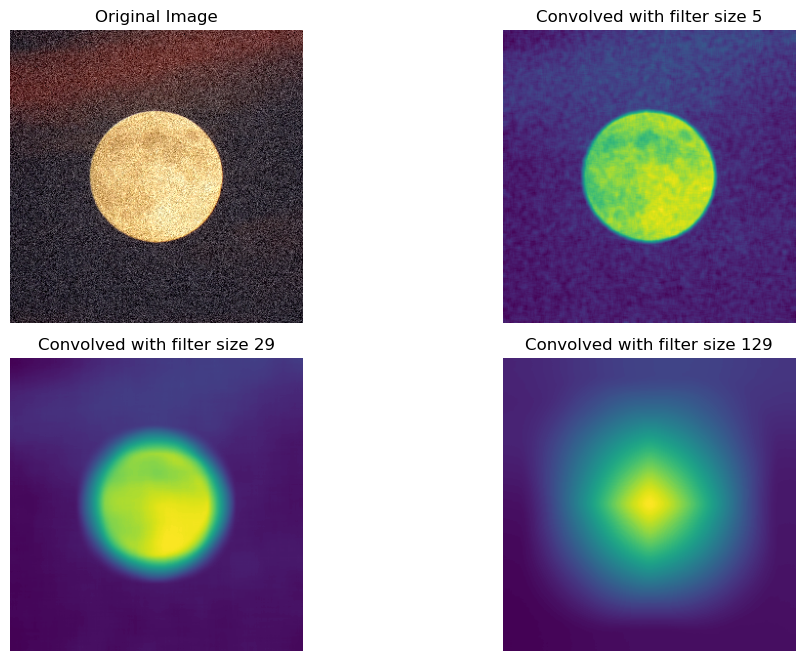
\includegraphics[width=1\linewidth]{convolved.png}
    \caption{The first image is the original image. }
    \label{conv}
\end{figure}
\subsection{Analysis of class FilteringAndBinarization(m)}
\noindent
\textbf{Purpose:} The \texttt{FilteringAndBinarization(m)} class provides image filtering (smoothing) and binarization (thresholding) utilities for grayscale or RGB images.

\vspace{0.3cm}
\textbf{Methods:}
\begin{itemize}[left=0pt]
    \item \textbf{box\_filter():} Returns an $m \times m$ averaging filter (used for smoothing).
    
    \item \textbf{convolve(image, kernel):} Converts input to grayscale if needed, then applies convolution using OpenCV (\texttt{cv2.filter2D}).\\
    \textbf{Time Complexity:} $\mathcal{O}(N \times M \times k^{2})$ for an $N \times M$ image and $k \times k$ kernel (but OpenCV is optimized).\\
    \textbf{Space Complexity:} $\mathcal{O}(N \times M)$ for the output image.
    
    \item \textbf{histogram\_compute(img):} Computes the normalized histogram of pixel intensities.\\
    \textbf{Time Complexity:} $\mathcal{O}(N \times M)$ for flattening and histogram calculation.\\
    \textbf{Space Complexity:} $\mathcal{O}(256)$ for histogram bins.
    
    \item \textbf{otsu\_binarization(norm\_histogram, threshold):} Calculates within-class variance for a given threshold using Otsu's method.\\
    \textbf{Time Complexity:} $\mathcal{O}(256)$ (since histogram bins are fixed).\\
    \textbf{Space Complexity:} $\mathcal{O}(1)$ (scalar values).
    
    \item \textbf{otsu\_threshold(img):} Finds the optimal threshold by minimizing within-class variance.\\
    \textbf{Time Complexity:} $\mathcal{O}(256)$ (calls \texttt{otsu\_binarization} for each possible threshold).\\
    \textbf{Space Complexity:} $\mathcal{O}(256)$ for storing variances.
\end{itemize}

\vspace{0.3cm}
\textbf{Specifications:}
\begin{itemize}[left=0pt]
    \item Handles both PIL images and NumPy arrays (RGB or grayscale).
    \item Uses OpenCV for fast convolution.
    \item Implements Otsu's method for automatic threshold selection.
    \item Designed for image preprocessing in segmentation and analysis tasks.
\end{itemize}

\vspace{0.3cm}
\textbf{Typical Workflow:}
\begin{center}
    \texttt{Filter image} $\rightarrow$ \texttt{Compute histogram} $\rightarrow$ \texttt{Find Otsu threshold} $\rightarrow$ \texttt{Binarize image}
\end{center}
\subsection{Analysis of Output}
\begin{itemize}
    \item \textbf{Small Filter Size ($5 \times 5$):} 
    \begin{itemize}
        \item Performs mild smoothing, reducing noise while preserving most image details.
        \item Object edges remain sharp and well-defined.
        \item Good for removing small-scale noise without significant blurring.
    \end{itemize}
    
    \item \textbf{Medium Filter Size ($29 \times 29$):} 
    \begin{itemize}
        \item Produces stronger smoothing, effectively reducing noise and local variations.
        \item Edges begin to blur, and fine textures are lost.
        \item Suitable for applications where denoising is more important than edge sharpness.
    \end{itemize}
    
    \item \textbf{Large Filter Size ($129 \times 129$):} 
    \begin{itemize}
        \item Performs heavy smoothing, leading to a very blurred image.
        \item Most fine details and textures are lost; the object shape becomes very diffused.
        \item Acts as a very strong low-pass filter, preserving only large-scale intensity changes.
    \end{itemize}
    
    \item \textbf{General Observation:} 
    \begin{itemize}
        \item Increasing filter size reduces noise but also causes loss of detail and edge sharpness.
        \item There is a trade-off between denoising and detail preservation; an optimal filter size must be chosen based on the application.
    \end{itemize}
\end{itemize}

Now, I will attach the graphs \cref{fig:thresholds} of within-class variances for various filter sizes and the optimal threshold for them. 
We can see that 
\begin{figure}[h!]
    \centering
    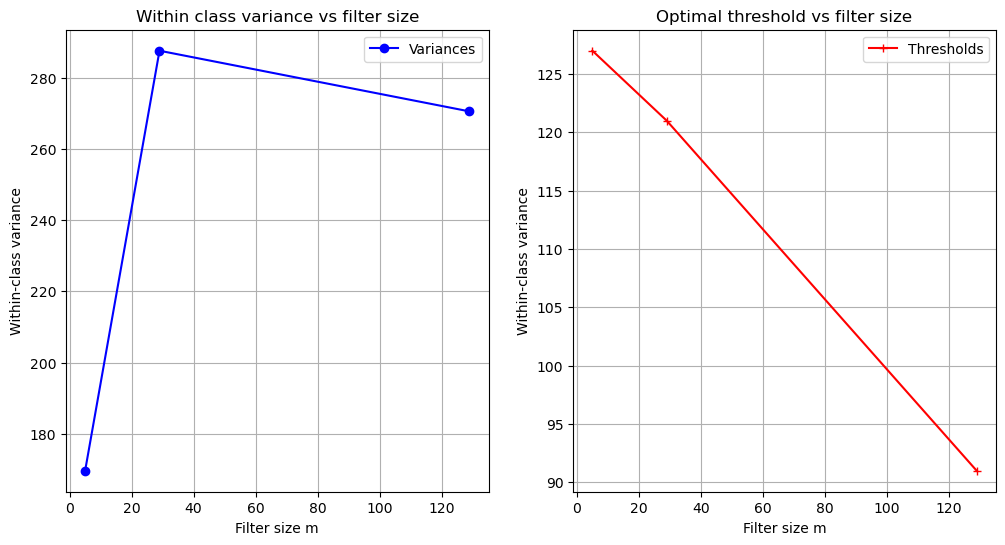
\includegraphics[width=1\linewidth]{thresholds.png}
    \caption{The left graph shows the within-class variance, and the right graph shows the optimal threshold corresponding to each m}
    \label{fig:thresholds}
\end{figure}

\begin{table}[h]
\centering
\caption{Within-Class Variance and Otsu Threshold for Different Filter Sizes}
\begin{tabular}{|c|c|c|}
\hline
\textbf{Filter Size ($m \times m$)} & \textbf{Within-Class Variance} & \textbf{Otsu Threshold} \\
\hline
$5 \times 5$   & $169.62$ & $127$ \\
$29 \times 29$ & $287.54$ & $121$ \\
$129 \times 129$ & $270.51$ & $91$ \\
\hline
\end{tabular}
\end{table}

The minimum within-class variance ($\sigma_w^{2*} $)is \textbf{169.62} for the filter size \textbf{$5 \times 5$}, indicating that this filter size achieves the best separation between foreground and background classes. The corresponding Otsu's threshold is \textbf{127}, which effectively binarizes the image by minimizing intra-class intensity variations while preserving important image details and edges. $\sigma_w^{2*} $ increases for some m and then starts decreasing. But the optimal threshold decreases monotonically. 

The graph \cref{fig:exp} shows the experimental result of $m_s$ and corresponding $\sigma_w^{2*} $ and $t^*$ 
\begin{figure}[b]
    \centering
    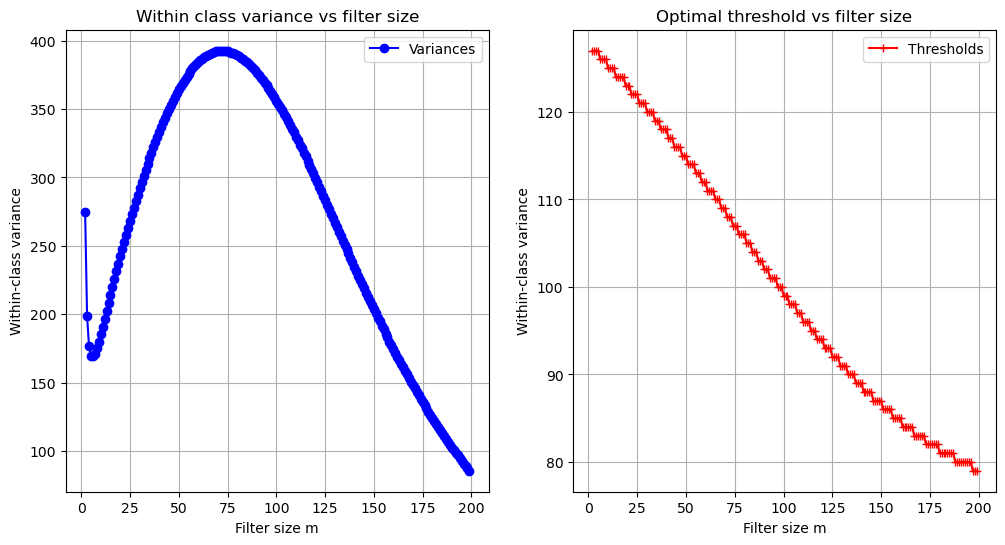
\includegraphics[width=1\linewidth]{exp.png}
    \caption{Graph of different m and corresponding $\sigma_w^{2*} $ and $t^*$ }
    \label{fig:exp}
\end{figure}

\clearpage
\begin{figure}[t]
    \centering
    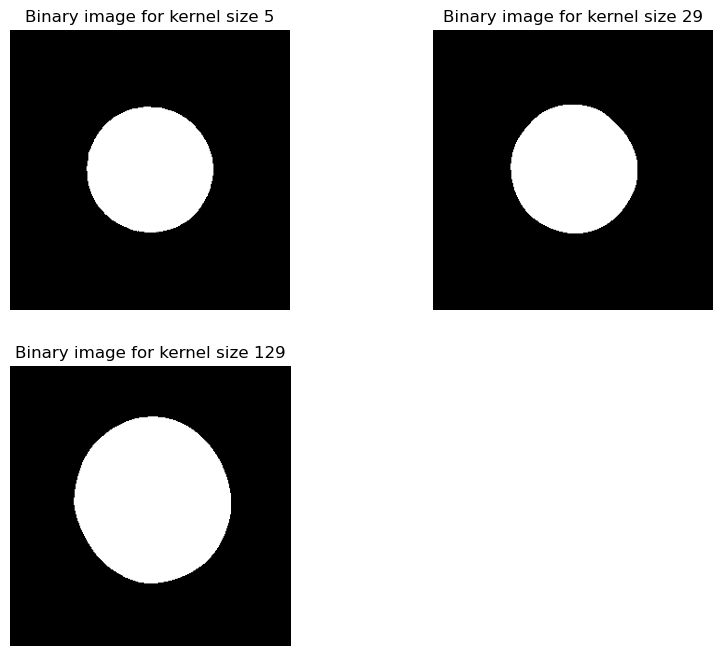
\includegraphics[width=0.5\linewidth]{bin_image.png}
    \caption{Binary images of filtered images with different filter(kernel) sizes}
    \label{bin_img}
\end{figure}
\begin{figure}[h]
    \centering
    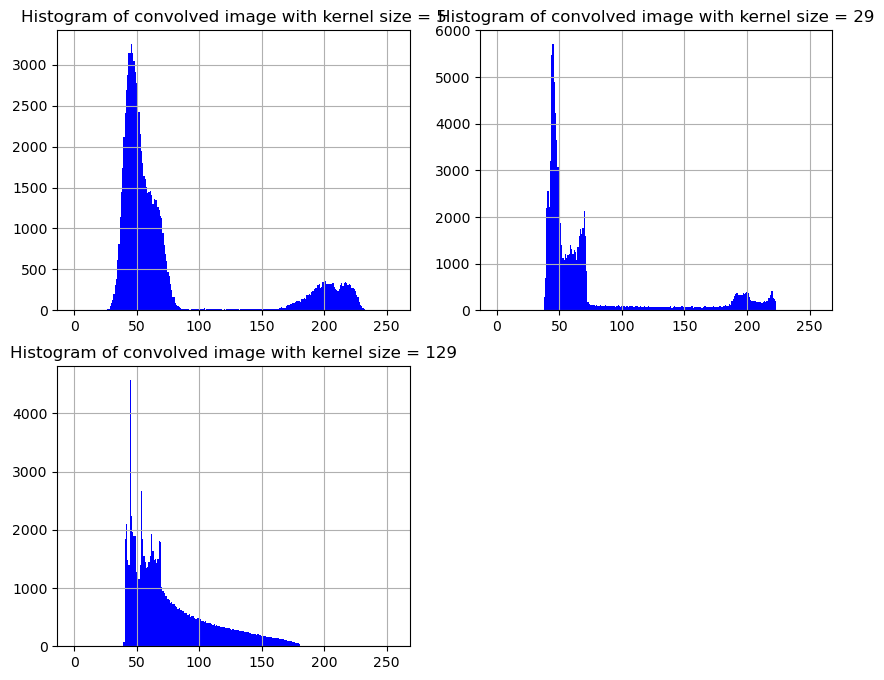
\includegraphics[width=0.6\linewidth]{hist.png}
    \caption{Histogram plots of different filtered images}
    \label{histograms}
\end{figure}
\noindent
The $\sigma_w^{2*} $ decreases for $m \in \{2,3,4,5\}$ and then increases for $m \in \{6,7...\cdots, 66\}$ and then continously decreases for $m \in \{67, \cdots 200\}$. 

\section{Scaling and Rotation with Interpolation:}
\textbf{Bilinear Interpolation:} Bilinear interpolation is used to compute an output pixel value based on a weighted average of its four nearest pixels. It is mainly used when scaling up an image, rotating it, or performing 3D rendering.

For upsampling and rotation, we can use a method called \textit{Nearest Neighbour Interpolation}, but it tends to produce undesirable artifacts, such as severe distortion of straight edges. For this reason, we don't use this method very frequently. 
Instead, we turn to \textit{Bilinear Interpolation}, which gives better results at the cost of a little computational overhead.  
Here is the approach for bilinear interpolation
\begin{figure}[h]
    \centering
    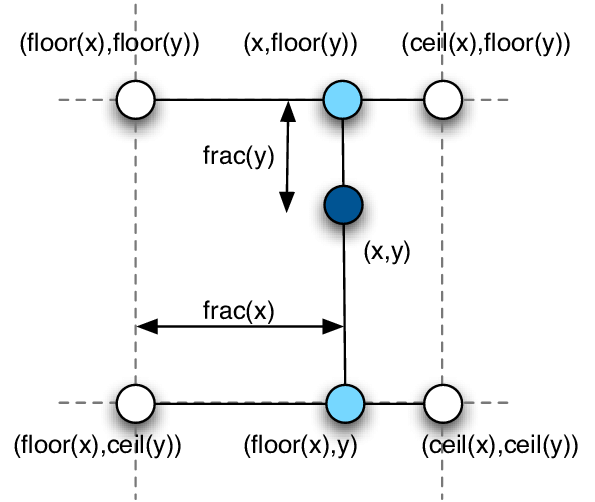
\includegraphics[width=0.5\linewidth]{bilinear.png}
    \caption{The figure showing the four nearest neighbours, using which we can estimate the intensity at the desired location}
    \label{fig:bilinear}
\end{figure}

\noindent
Assume the four neighboring pixels are $(x_0, y_0), (x_0, y_1), (x_1, y_0), \text{and} (x_1, y_1)$ with corresponding intensities $I_a, I_b, I_c,$ and $I_d$.  
Let 
\[
dx = x - \lfloor x \rfloor, \qquad dy = y - \lfloor y \rfloor
\]
denote the fractional parts of $x$ and $y$.  
Then the intensity at $(x,y)$ using bilinear interpolation is given by \cref{eq:bilinear}

\begin{equation}
I(x,y) = I_a (1 - dx)(1 - dy) + I_b (1 - dx)dy + I_c dx(1 - dy) + I_d dx dy.
\label{eq:bilinear}
\end{equation}

\noindent
Note that each weight in \cref{eq:bilinear} is proportional to the distance from the \emph{opposite} pixel location. 
For example, the coefficient of $I_a$ is $(1 - dx)(1 - dy)$, which assigns a higher weight to $I_a$ when $(x,y)$ is closer to $(x_0, y_0)$ and a lower weight as $(x,y)$ moves away. 
Similarly, the other coefficients $(1 - dx)dy$, $dx(1 - dy)$, and $dxdy$ assign weights to $I_b, I_c,$ and $I_d$ based on their relative proximity to $(x,y)$. 
Thus, bilinear interpolation performs a weighted average where weights decrease linearly with distance from each neighboring pixel.

\noindent
Here is the result of upsampling [\ref{fig:upAndRot}] and then rotation on the flower image. 
\begin{figure}[h]
    \centering
    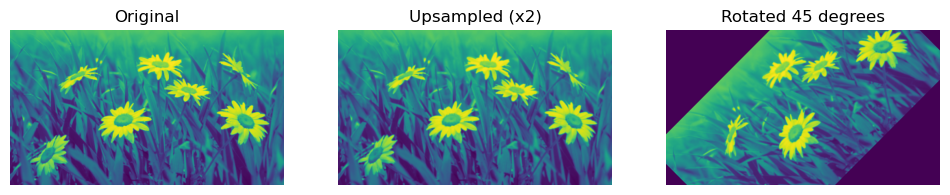
\includegraphics[width=1\linewidth]{upAndRot.png}
    \caption{The original image first upsampled $(\times 2)$ and rotated by $45^o$ counter-clockwise}
    \label{fig:upAndRot}
\end{figure}

Figure [\ref{Figure:rotAndUp}] is the result of rotation  and then upsampling on the flower image
\begin{figure}[h]
    \centering
    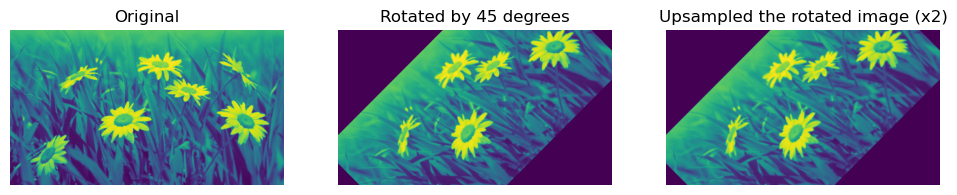
\includegraphics[width=1\linewidth]{rotAndUp.png}
    \caption{The original image first rotated by $45^o$ counter-clockwise and then upsampled $\times 2$}
    \label{Figure:rotAndUp}
\end{figure}

Later, we computed the difference between the two final images. And the minimum of the difference is 0.00, and the maximum of the difference is 255.00. Also, I will attach the resulting image \ref{diff} we got.
\begin{figure}[h!]
    \centering
    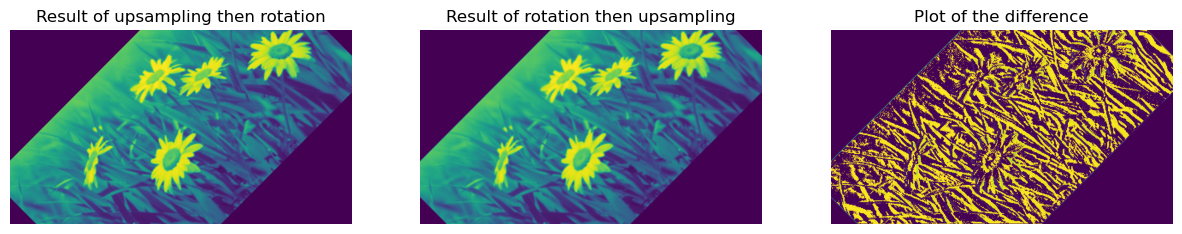
\includegraphics[width=1\linewidth]{diff.png}
    \caption{The left image shows upsample $\rightarrow$ rotation. The middile image shows rotation $\rightarrow$ upsample and the right image shows the difference of the two.}
    \label{diff}
\end{figure}

\subsection{Analysis of the results}
\begin{enumerate}[label = (\alph*)]
    \item \textbf{Upsample and Rotation}
    \begin{itemize}
    \item \textbf{Upsample (×2):} Enlarges the image while keeping full rectangular coverage. The resolution is effectively increased.

    \item \textbf{Rotate by 45°} Now the enlarged image is rotated, but the black corners occupy relatively less of the frame, since the image is bigger before rotation. Interpolation smoothness looks better, too.
    \end{itemize}
    \item \textbf{Rotation and Upsampling}
    \begin{itemize}
        \item \textbf{Rotate by 45°:}  Produces a diamond-shaped image inside a rectangular frame (black corners due to rotation).
        \item \textbf{Upsample (×2):} Magnifies the rotated image. The black corners also get enlarged, and interpolation artifacts may be more noticeable.
    \end{itemize}
    \item \textbf{Order of operations matters:}
    \begin{itemize}
        \item Rotate → Upsample: magnifies the rotated frame (including empty black regions). Artifacts become more visible.
        \item Upsample → Rotate: preserves more detail from the original image, and the black borders are proportionally smaller.
    \end{itemize}
\end{enumerate}
The operations are not commutative. The output depends on the order, so the results are \textbf{NOT Identical}.

\section{Image Sharpening Concept:}

For this question, I have used the concept of \textit{unsharp masking} to sharpen the image. To acheive the desired result, we subtract the unsharp (blurred) version of the image. This process is called \textit{unsharp masking}. The steps, we followed are the following
\begin{enumerate}
    \item Blur the original image
    \item Subtract the blurred image from the original (the resulting difference is
called the mask.)
    \item Add the mask to the original.
\end{enumerate}

\begin{equation}
g_{\text{mask}}(x,y) = f(x,y) - \overline{f}(x,y),
\end{equation}
where $\overline{f}(x,y)$ denotes the blurred (or smoothed) version of $f(x,y)$.
\begin{equation}
    g(x,y) = f(x,y)  + kg_{mask}(x,y)
\end{equation}
\[
g(x,y) = f(x,y) + k[f(x,y)-\overline{f}(x,y)]
\]
\begin{equation}
    g(x,y) = (1+k)f(x,y) -k\overline{f}(x,y)
\end{equation}
\noindent
If $k=1$, then we call it unsharp masking, and if $k>1$, then high-boost filtering. For $k<1$, it de-emphasizes the contribution of the unsharp mask. 
The figure [\ref{unsharp}] shows how we get a sharpened image using unsharp masking.
For, blurring the image, I have a Gaussian filter with different $\sigma$
\subsection{Analysis of results}
\begin{itemize}
    \item For $p=0.5$, Edges and fine details are enhanced, but not aggressively. A good balance between clarity and naturalness.
    \item High-frequency components are fully added back. Edges are crisp, but risk of haloing or noise amplification increases.
\end{itemize}
\subsection{Conclusion}
\begin{enumerate}
    \item With $p=0$, we don't see any change, or we see the original image.
    \item Higher $p$ values can introduce negative pixel values, especially near low-intensity regions.
    \item These may cause dark halos around edges, which can be visually objectionable or misleading in diagnostic imaging.
\end{enumerate}
\begin{figure}[h]
    \centering
    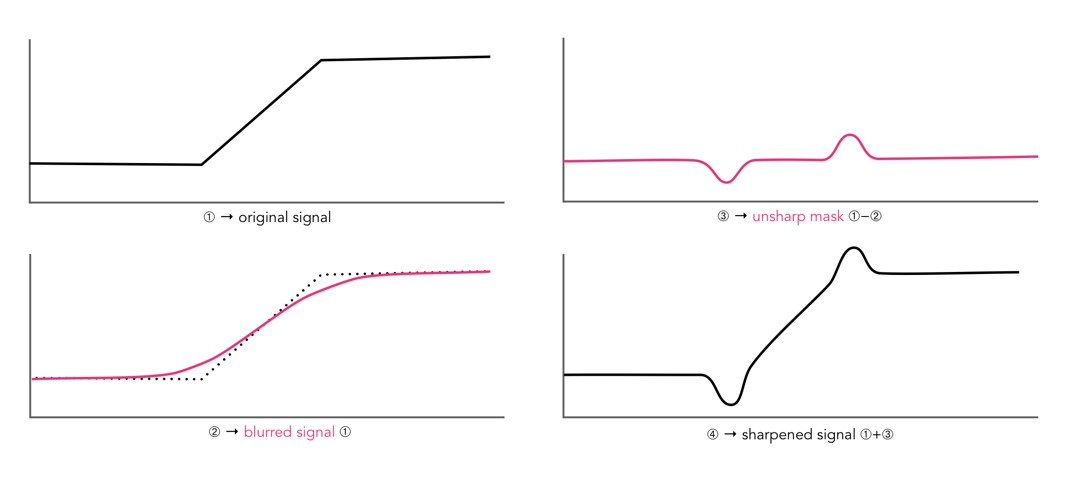
\includegraphics[width=1\linewidth]{unsharp.png}
    \caption{1D-Illustration of the mechanics of unsharp masking.}
    \label{unsharp}
\end{figure}

I will attach a few results of sharpening. 
\begin{figure}[h]
    \centering
    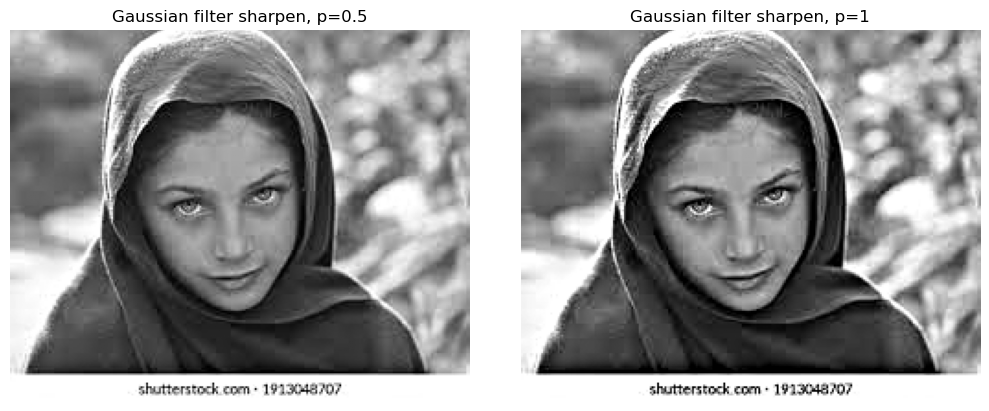
\includegraphics[width=0.75\linewidth]{girl.png}
    \caption{Girl image before and after sharpening}
    \label{fig:placeholder}
\end{figure}
\begin{figure}
    \centering
    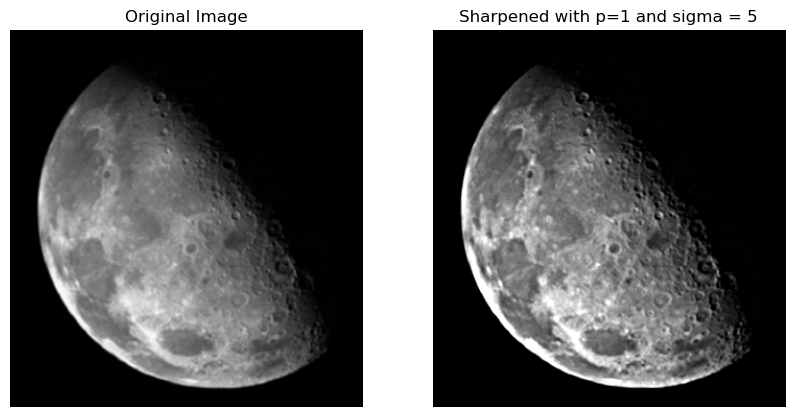
\includegraphics[width=0.5\linewidth]{earth.png}
    \caption{Earth image before and after sharpening}
    \label{fig:placeholder}
\end{figure}
\begin{figure}
    \centering
    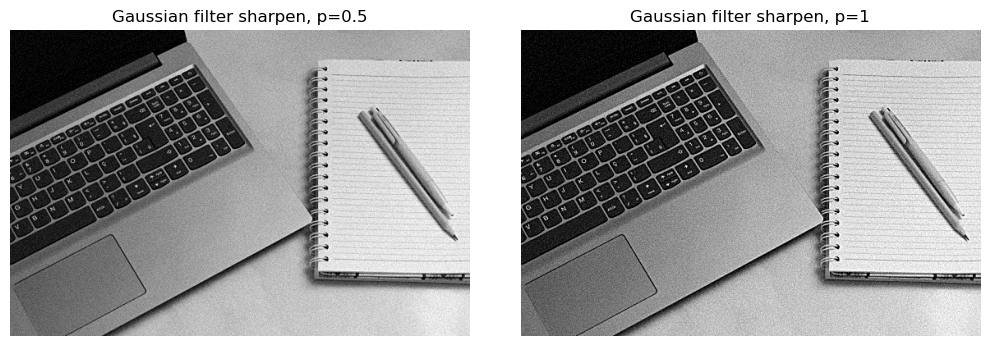
\includegraphics[width=1\linewidth]{study.png}
    \caption{Sharpening with p=0.5 and p=1}
    \label{fig:placeholder}
\end{figure}

\begin{figure}
    \centering
    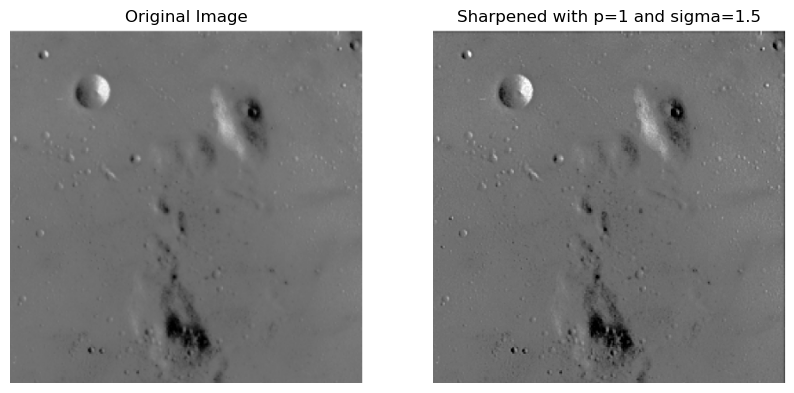
\includegraphics[width=1\linewidth]{land.png}
    \caption{Earth image before and after applying sharpening}
    \label{fig:placeholder}
\end{figure}

\begin{figure}[t]
    % \centering
    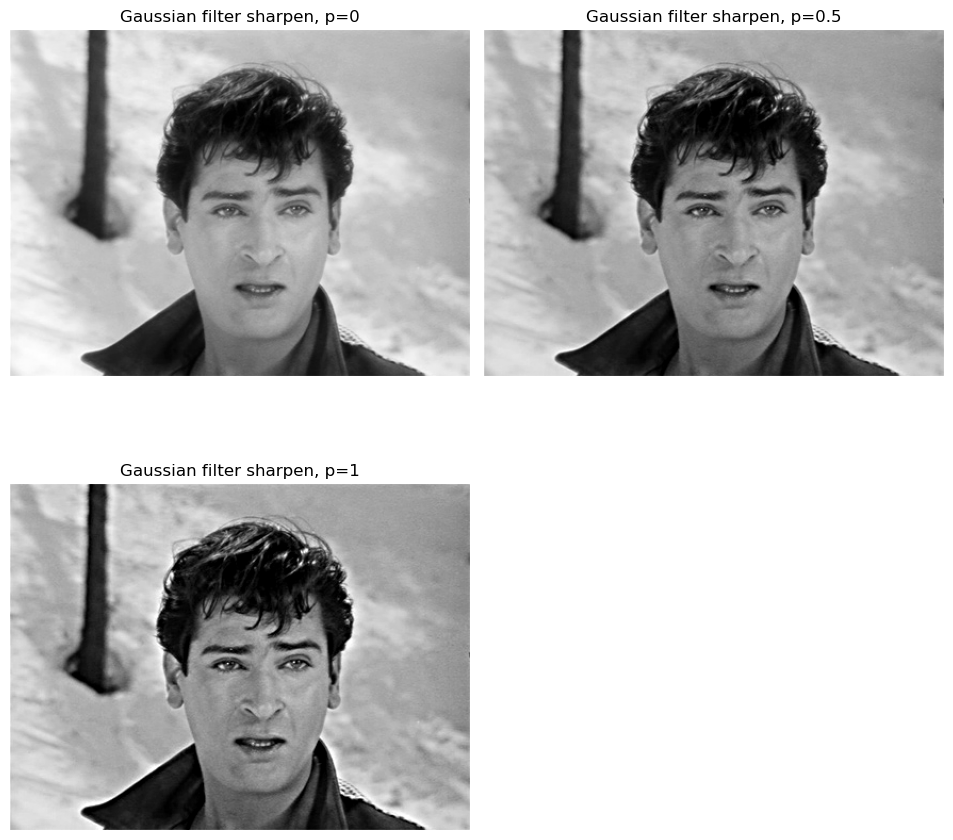
\includegraphics[width=1\linewidth]{rajesh.png}
    \caption{Image of an Indian actor before and after applying sharpening}
    \label{fig:placeholder}
\end{figure}

\section{Conclusion}
\begin{enumerate}
    \item \textbf{Spatial Filtering and Binarization} Through box blurring and Otsu’s thresholding, we observed how varying filter sizes influence image smoothness and segmentation quality. The optimal filter size minimized within-class variance $\sigma_w^2$, highlighting the trade-off between noise suppression and edge preservation in preprocessing pipelines.
    \item \textbf{Interpolation and Geometric Transformations} The comparison between scaling-then-rotation versus rotation-then-scaling revealed that interpolation order significantly affects pixel distribution and visual fidelity. The difference image underscored how transformation sequencing can introduce subtle artifacts, which are critical in precision-sensitive domains like medical imaging.
    \item \textbf{Sharpening with Adjustable Intensity:} 
    The \texttt{sharpenAdjust(img, p)} function demonstrated how controlled 
    enhancement via parameter $p$ can improve edge clarity while managing halo artifacts. 
    Testing across multiple images confirmed that moderate sharpening 
    (e.g., $p=0.5$) offers a balanced improvement without compromising visual integrity.

    
\end{enumerate}

\end{document}
